%%%% Proceedings format for most of ACM conferences (with the exceptions listed below) and all ICPS volumes.
\documentclass[sigconf]{acmart}
\usepackage{tikz}
%%%% As of March 2017, [siggraph] is no longer used. Please use sigconf (above) for SIGGRAPH conferences.

%%%% Proceedings format for SIGPLAN conferences 
% \documentclass[sigplan, anonymous, review]{acmart}

%%%% Proceedings format for SIGCHI conferences
% \documentclass[sigchi, review]{acmart}

%%%% To use the SIGCHI extended abstract template, please visit
% https://www.overleaf.com/read/zzzfqvkmrfzn

\begin{document}

\title{Higher-order networks: Exploring air traffic dynamics}

% The "author" command and its associated commands are used to define the authors and their affiliations.
\author{Bradley Dice}
\email{bdice@bradleydice.com}
\orcid{0000-0002-9983-0770}
\affiliation{
  \institution{University of Michigan \\ Department of Physics}
  \city{Ann Arbor}
  \state{Michigan}
  \postcode{48109}
}

\author{Daniel McCusker}
\email{dmccuske@umich.edu}
\affiliation{
  \institution{University of Michigan \\ Applied Physics}
  \city{Ann Arbor}
  \state{Michigan}
  \postcode{48109}
}

\author{Shannon Moran}
\email{moranse@umich.edu}
\orcid{0000-0002-3579-3149}
\affiliation{
 \institution{University of Michigan \\ Department of Chemical Engineering}
  \city{Ann Arbor}
  \state{Michigan}
  \postcode{48109}
 }

\renewcommand{\shortauthors}{Dice, et al.}

% The abstract is a short summary of the work to be presented in the article.
% \begin{abstract}
% \end{abstract}

% Show author, affiliation, and title information
\maketitle

% \section{Guidelines}
% Length: 4-5 pages
% \begin{itemize}
%     \item Section 2. Data: Describe the synthetic and real data that you will use, and explain the data collection process (if applicable).
%     \item Section 3. Proposed Method: Introduce the method that you propose, give the necessary definitions, potentially give proof of concept.
%     \item Section 4. Experiments: Give some preliminary experiments (on synthetic or real data).
%     \item Section 5. Progress and Next Steps (temporary section): Outline your next steps and whether you are on track. Now that you have had time to work on your projects, if anything has changed with respect to your proposal, mention it.
%     \item Section 6. Division of work (your grade will depend on your contribution to the project)
% \end{itemize}

\section{Midterm Summary}
In this project, we proposed studying trajectory data to explore higher-order network representations. We considered available data sets and settled on an air traffic data set, which has previously been used as a model system in the literature \cite{Rosvall2014}. As of this midterm report, we have developed a pipeline for data extraction and transformation into parsable trajectories, and have built and analyzed both first order and higher-order networks (HONs) for a subset of the data (Q1 2011). We detail this progress in the Experimental section. We will next extend this work to the full data set from 1993-2018. The core piece of our proposal was implementing a community detection algorithm on the HONs. In a slight expansion on the original proposal scope in response to feedback, we plan to implement multiple community detection algorithms to compare the resulting communities identified in HONs with each method. Overall, we are on track to deliver the project scoped in our proposal.

% =====
% DATA
% =====

\section{Data: Airline traffic data}

\subsection{Data choice and collection}
We chose data from the Airline Origin and Destination Survey (DB1B), collected by the Office of Airline Information of the Bureau of Transportation Statistics. We made this choice due to the quality of the data, consistency of collection (1993--2018), and its previous use as a model data set by other papers in the field \cite{AirlineData}. This database contains three primary data views: \textit{Coupon}, \textit{Market}, and \textit{Ticket}, aggregated on a quarterly basis from 1993 Q1 to 2018 Q3. This includes 837 million observations of itinerary coupons, 507 million observations of origin/destination markets, and 286 million observations of airline tickets.

We successfully downloaded and imported this data into Python \texttt{pandas} dataframes (only one quarter of data per dataframe for visualization). The data appear to be clean (no \texttt{NaN} values) with few outliers (e.g. one itinerary that had over 900 passengers on it - sounds like a party!).

We determined the following, after cross-referencing with a number of airline industry sources:\footnote{https://www.iata.org/policy/Documents/coupon-use-paper.pdf}
\begin{itemize}
    \item \textbf{Coupons} represent individual boarding passes, e.g. one leg from LGA-DTW. This is the data set we ultimately use, as described below.
    \item \textbf{Tickets} represent collections of Coupons. A round trip ticket from DTW-LHR via JFK would be a ticket composed of 4 Coupons: DTW-JFK, JFK-LHR, LHR-JFK, and JFK-DTW. To get this trajectory, we need to join the Coupons data based on a ticket ID. As a result, we did not need to use the Tickets database except to spot-validate that our data interpretation was correct.
    \item \textbf{Markets} represent journey segments that are separated by a break in the travel. For example, a round-trip ticket to a conference and back would be composed of two markets. The first market is the series of flights (including layovers) on the way to the conference, followed by a break in travel (for the conference). The second market is the return portion of the trip, ending in the traveler coming home. One-way tickets are composed of only one market, whereas multi-city flights purchased on the same ticket could have three or more markets. We are interested in including travel irrespective of markets, so this data set is not useful to us. %Not all airlines participate in all markets. As an example, DTW-MDW is a segment that is served by Southwest and Delta, but not by American. A ``market" can be analyzed by average price of ticket, traffic, etc. After investigation, we will not be using this data set.
\end{itemize}

The raw DB1B Coupon data gathered from the Bureau of Transportation Statistics contains 35 columns with a primary key for the coupon, foreign keys for linking coupon data to data in the Ticket and Market database, and a number of fields describing that coupon (e.g. origin and destination airports, various metadata).

\subsection{Data management with \texttt{signac}}
Because there are over 100 quarters of data, we needed an organizational scheme that would offer the flexibility to rapidly experiment on one quarter and automate our operations as we scale to the full data set. To do this, we use the open-source \texttt{signac} framework (\url{https://signac.io}). The project workflow script performs operations on each quarter of data using a directed graph of tasks with pre- and post-conditions. In this case, the operations graph (Figure \ref{fig:operations}) runs the entire workflow, from downloading raw data through processing with PySpark. The entire operations graph is run for each quarter of data, and each operation can be run in serial or parallel depending on memory requirements.

While we were able to load one quarter of one year of data into a \texttt{pandas} dataframe, analyzing multiple quarters (as we intend!) required expanding to use PySpark\footnote{https://spark.apache.org/docs/latest/api/python/index.html}, as we planned in our proposal. PySpark is compatible with Hadoop (and all analysis has been run on \texttt{flux-hadoop} to date) but is easier to program than Hadoop because it has the concept of \texttt{DataFrame}s. Staying in Python also means that it is easier to rapidly prototype algorithms and utilize Jupyter notebooks for processing data. Operations were prototyped interactively in Jupyter notebooks, configured to interface with the Spark cluster in a real-time session, and then ported into the \texttt{signac-flow} project workflow script. Smaller pre- and post-processing tasks utilized \texttt{pandas}. All jobs (\texttt{bash}, Python, \texttt{pandas}, PySpark) were run using \texttt{signac-flow}. The entire workflow (downloading input data, parsing and pre-processing, Spark submission, and analysis) can be reproduced or re-run by calling one terminal command.

\begin{figure}
    \centering
    \tikzset{every picture/.style={line width=0.75pt}} %set default line width to 0.75pt        

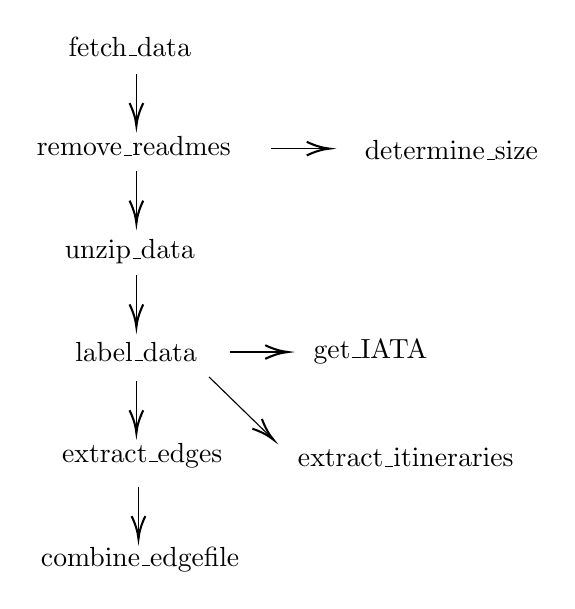
\begin{tikzpicture}[x=0.75pt,y=0.75pt,yscale=-1,xscale=1]
%uncomment if require: \path (0,300); %set diagram left start at 0, and has height of 300

%Straight Lines [id:da774937353877323] 
\draw    (329.2,28.2) -- (329.2,51.2) ;
\draw [shift={(329.2,53.2)}, rotate = 270] [color={rgb, 255:red, 0; green, 0; blue, 0 }  ][line width=0.75]    (10.93,-3.29) .. controls (6.95,-1.4) and (3.31,-0.3) .. (0,0) .. controls (3.31,0.3) and (6.95,1.4) .. (10.93,3.29)   ;

%Straight Lines [id:da37948328121331465] 
\draw    (329.2,75.2) -- (329.2,98.2) ;
\draw [shift={(329.2,100.2)}, rotate = 270] [color={rgb, 255:red, 0; green, 0; blue, 0 }  ][line width=0.75]    (10.93,-3.29) .. controls (6.95,-1.4) and (3.31,-0.3) .. (0,0) .. controls (3.31,0.3) and (6.95,1.4) .. (10.93,3.29)   ;

%Straight Lines [id:da2604231609644325] 
\draw    (394.2,64.2) -- (420.2,64.2) ;
\draw [shift={(422.2,64.2)}, rotate = 180] [color={rgb, 255:red, 0; green, 0; blue, 0 }  ][line width=0.75]    (10.93,-3.29) .. controls (6.95,-1.4) and (3.31,-0.3) .. (0,0) .. controls (3.31,0.3) and (6.95,1.4) .. (10.93,3.29)   ;

%Straight Lines [id:da5664873603541694] 
\draw    (329.2,125.2) -- (329.2,148.2) ;
\draw [shift={(329.2,150.2)}, rotate = 270] [color={rgb, 255:red, 0; green, 0; blue, 0 }  ][line width=0.75]    (10.93,-3.29) .. controls (6.95,-1.4) and (3.31,-0.3) .. (0,0) .. controls (3.31,0.3) and (6.95,1.4) .. (10.93,3.29)   ;

%Straight Lines [id:da979436082222915] 
\draw    (374.2,162.2) -- (400.2,162.2) ;
\draw [shift={(402.2,162.2)}, rotate = 180] [color={rgb, 255:red, 0; green, 0; blue, 0 }  ][line width=0.75]    (10.93,-3.29) .. controls (6.95,-1.4) and (3.31,-0.3) .. (0,0) .. controls (3.31,0.3) and (6.95,1.4) .. (10.93,3.29)   ;

%Straight Lines [id:da2369337782591805] 
\draw    (329.2,176.2) -- (329.2,199.2) ;
\draw [shift={(329.2,201.2)}, rotate = 270] [color={rgb, 255:red, 0; green, 0; blue, 0 }  ][line width=0.75]    (10.93,-3.29) .. controls (6.95,-1.4) and (3.31,-0.3) .. (0,0) .. controls (3.31,0.3) and (6.95,1.4) .. (10.93,3.29)   ;

%Straight Lines [id:da5287233692241446] 
\draw    (330.2,227.2) -- (330.2,250.2) ;
\draw [shift={(330.2,252.2)}, rotate = 270] [color={rgb, 255:red, 0; green, 0; blue, 0 }  ][line width=0.75]    (10.93,-3.29) .. controls (6.95,-1.4) and (3.31,-0.3) .. (0,0) .. controls (3.31,0.3) and (6.95,1.4) .. (10.93,3.29)   ;

%Straight Lines [id:da33374672983323517] 
\draw    (364.2,174.2) -- (393.77,203) ;
\draw [shift={(395.2,204.4)}, rotate = 224.25] [color={rgb, 255:red, 0; green, 0; blue, 0 }  ][line width=0.75]    (10.93,-3.29) .. controls (6.95,-1.4) and (3.31,-0.3) .. (0,0) .. controls (3.31,0.3) and (6.95,1.4) .. (10.93,3.29)   ;


% Text Node
\draw (326,15) node  [align=left] {fetch\_data};
% Text Node
\draw (328,63) node  [align=left] {remove\_readmes};
% Text Node
\draw (481,65) node  [align=left] {determine\_size};
% Text Node
\draw (326,114) node  [align=left] {unzip\_data};
% Text Node
\draw (329,162) node  [align=left] {label\_data};
% Text Node
\draw (442,162) node  [align=left] {get\_IATA};
% Text Node
\draw (332,212) node  [align=left] {extract\_edges};
% Text Node
\draw (331,262) node  [align=left] {combine\_edgefile};
% Text Node
\draw (459,213) node  [align=left] {extract\_itineraries};


\end{tikzpicture}
    \caption{Operations graph implemented in \texttt{signac-flow}.}
    \label{fig:operations}
\end{figure}

\subsection{Data transformation into networks}
Transforming this data from massive CSV files into first-order and HON networks required two different operations. For the first-order network, we represented the data as a weighted directed graph. The coupons were parsed to extract origin and destination airports, and the total number of coupons grouped by each origin/destination pair was summed to give a weight for the (origin, destination) directed edge in the graph. For the higher-order network, coupons were grouped by their ticket's unique identifier so that a series of airports could be constructed for each ticket. This led to two PySpark operations with different output formats.

% =====
% METHODS
% =====
\section{Proposed Methods}
% Introduce the method you propose, give the necessary definitions, and potentially give proof of concept.

Our project relies upon the following methods, which increase in order of complexity.

\begin{enumerate}
    \item Build first order network from coupon data 
    \item Build a higher-order network (HON) from compiled trajectory data
    \item Implement community detection on HONs: InfoMap versus motif-based community detection
\end{enumerate}

\subsection{Build first order network from coupon data}
We build weighted directed first order networks from the coupon trajectories compiled from the raw data as outlined in the ``Data'' section. As a note, we could also weight by the total number of \textit{passengers} on each edge, but since most (>75\%) of coupons are only one passenger, we decided this was an incremental update we did not need.

\subsection{Build a higher-order network (HON) from compiled trajectory data}
First, coupons were merged by their itinerary's unique identifier to form trajectories. These trajectories are the input for the \texttt{BuildHON+} algorithm. Previous work on DB1B data by Rosvall et al. made some assumptions about paths' endpoints (e.g. choice of memory nodes) that make the problem simpler and capture helpful dynamics \cite{Rosvall2014}. Specifically, the first and last airports on a ticket are included twice to enforce the inclusion of self-memory nodes that reinforce the importance of a home city over transfer traffic. This will also make our analysis more comparable to the literature result.

We use the improved \texttt{BuildHON+} algorithm of Xu et al. \cite{Xu2017} to build a higher-order network of this data. There is an open-source Python implementation\footnote{https://github.com/xyjprc/hon} that we used for analysis\cite{Xu2016,Xu2017}. For now, we have allowed the algorithm to dynamically choose its own cutoff order $k$ for each trajectory history by setting a large maximum value ($k = 99$). The algorithm's time complexity is not strongly dependent on $k$ after a certain point, as seen in Table 1 of the HON paper where the run time of $k = 3$ and $k = 5$ differ by only 8\% \cite{Xu2016}. This is because there are typically far fewer correlations of high order than low order, so testing correlations of order $k$ for extension to order $k+1$ gets cheaper as the number of correlations decreases.

\subsection{Implement community detection on HONs: InfoMap versus motif-based detection}
We'd like to follow up on the proposal feedback, which asked how we were going to evaluate the quality of the communities we find. Our first metric would be ``accuracy'' relative to the communities identified by Rosvall et al. \cite{Rosvall2014}. However, we do not have explicit information about the airport-to-community mappings identified in that work; we have only a few representative samples.

Instead, we've decided to compare the relative ``performance'' of different community detection methods. This exercise will thus give us an opportunity to explore the relative strengths and weaknesses of these methods.

First we plan to implement InfoMap, a random walker-based (MapEquation) community detection algorithm, to detect overlapping communities in the airport nodes \cite{Rosvall2009}. This will allow us to directly compare our results to the fixed second-order airline representation and expand it to $k$-order representations \cite{Rosvall2014}. An additional advantage of this approach is that there is already an available implementation in \texttt{C++} and Python, which we expect to be able to leverage in part.\footnote{https://github.com/mapequation/infomap}

A method that has been used to identify \textit{clusters} in higher-order networks is based on motif detection \cite{Benson2016}. In this algorithm, clusters are built to minimize the number of a given motif that are cut when an edge is removed. Code is available in MATLAB and will need to be translated to Python for our project\footnote{https://github.com/arbenson/higher-order-organization-matlab}. While this method has been applied to higher-order networks, it has never been applied to data of this scale and to transportation data specifically. There is a simple example of traffic data that was analyzed, though is not directly analogous. In addition, the authors assert that this can also be used to identify communities -- but we need to explore further whether this claim is justified.

There is a \textbf{medium-risk} that this approach simply will not work for our data, but we are excited to explore it as this work has come up repeatedly in our review of the literature. We want to be very clear that this is an incremental ``bonus'' on top of our already-proposed work, and is a risky endeavor. We are going to make a good faith effort to complete it in four weeks but are not confident that it will be a clear success.

One might ask why we are not using another community detection algorithm discussed in class. In part, this is because performance for InfoMap is already benchmarked against the Louvain method and we were looking to do something more ``novel'' than replicating this particular work on the airport traffic network \cite{Rosvall2014}. Additionally, the motif-based method had been discussed at several points in our literature review (and Benson, the lead author, has a PhD thesis which was very helpful introductory material for us), and we are excited to try implementing it in Python and applying it to our networks.

% =====
% EXPERIMENTS
% =====
\section{Experiments}
% Give some preliminary experiments (on synthetic or real data).
Here, we have framed each stage of our project as an ``experiment.'' Our implicit hypothesis, unless otherwise stated, is that we will be able to generate findings that are reasonable -- e.g. found in the literature on comparable data sets \cite{Rosvall2014}, or explainable by cross-referencing with common-sense analyses of airline data.

\subsection{Experiment 1: Creating networks from flight trajectories}
\textbf{Hypothesis}: We can represent airline flights as a first-order network using the coupon data. These networks will demonstrate a hub-and-spoke model, but will not preserve trajectory information.

\begin{figure}
    \centering
    \includegraphics[width=0.5\textwidth]{first_order_network.png}
    \caption{Shown is a best-possible visualization for the first-order network built using the trajectories compiled from the available coupon data for Q1 2011. This is a low-diameter network (average shortest path length of 2.36), and it is apparent from this representation that an alternative (in this case, higher-order) approach is needed to glean meaningful insights from the data.}
    \label{fig:first_order}
\end{figure}

Contrasting our initial hypothesis, we do not actually see a hub-and-spoke model. Instead, the system is highly connected and shows an average shortest path length of 2.361, as illustrated in Figure \ref{fig:first_order}. We hypothesize that individual airlines may look more like a hub-and-spoke but because this data reflects the combination of many airlines, we observe a dense core with very few nodes at the periphery.

\subsection{Experiment 2: Comparing higher-order network representations with PageRank}
\textbf{Hypothesis}: A higher-order network will change the PageRank scores of some airports relative to the first-order representation. This will indicate that there is additional information embedded in the higher-order representation.

\begin{figure*}[t]
    \centering
    \includegraphics[width=\textwidth]{PageRank_fon_map.png}
    \caption{Nodes identified from the data set over period Q1 2011. Node size and color corresponds to the node's PageRank value based on a first order network, i.e. one that does not take higher-order dependencies into account.}
    \label{fig:fon-map}
\end{figure*}

\begin{figure*}[t]
    \centering
    \includegraphics[width=0.9\textwidth]{pagerank_demo.png}
    \caption{Airports showing the largest change in PageRank between first-order and $k$-order network representations built for Q1 2011 data. Discussion in the text.}
    \label{fig:pagerank_changes}
\end{figure*}

\begin{table}[tb]
\begin{tabular}{c|c|c|c}
First-order  &                &   Higher-order &                \\
\hline
Airport Code & PageRank Score &   Airport Code & PageRank Score \\
\hline
ATL          & 0.088  &   ATL          & 0.107   \\
CLT          & 0.051  &   ORD          & 0.060  \\
DFW          & 0.047  &   CLT          & 0.059  \\
DEN          & 0.047   &   DFW         & 0.059  \\
ORD          & 0.046  &   DEN          & 0.054
\end{tabular}
\caption{Top five PageRanked airports for first-order and variable ($k$) higher-order networks.}
\label{tab:pagerank}
\end{table}

We visualize the results of our PageRank analysis for a first-order network in Figure \ref{fig:fon-map}. The result verifies our intuitions about which airports are major hubs: Atlanta, Chicago, Denver, LA, Philadelphia, etc. PageRank values for the five airports with the largest PageRank values calculated for the first-order and $k$-order representations are shown in Table \ref{tab:pagerank}.

In Figure \ref{fig:pagerank_changes}, we highlight the ten airports that see the largest increase in PageRank when comparing $k$-order networks to first-order networks, as well as the ten airports that see the largest decreases. Both of these populations are composed of ``hubs'', while smaller airports are largely unchanged after accounting for higher-order dependencies (not shown in this report, but analysis is available).

We can take away from these results that a $k$-order HON representation is adding some amount of value and information to these network analyses. However, we will need to do more work to understand and build our intuition for why hubs are the airports whose PageRanks are most impacted by this improved representation. Our current hypothesis is that these hubs have the largest absolute PageRanks, and therefore even a minor percentage change in the PageRank taking into account higher-order dependencies would be a larger absolute change for hubs than minor airports.

% ======
% PROGRESS AND NEXT STEPS
% ======
\section{Progress and next steps}
% Outline your next steps and whether you are on track. Now that you have had time to work on your projects, if anything has changed with respect to your proposal, mention it.

\begin{figure}[t]
    \centering
    \includegraphics[width=0.5\textwidth]{gantt.png}
    \caption{Gantt chart illustrating progress to date (underlined, in red) and remaining work. Our team remains on track to complete the work outlined in our proposal.}
    \label{fig:gantt}
\end{figure}

Our major tasks are outlined in the Gantt chart in Figure \ref{fig:gantt}. Over the next four weeks, we will primarily focus on analysis of the HONs we have now successfully built. We are currently planning on implementing two different types of community detection, as outlined in the Proposed Methods. We are confident that given our progress over the last 3 weeks, this is an achievable goal. There is some risk that the expanded scope of community detection into motif-based approaches will be unsuccessful, but this was not part of the original proposal. We are on track to complete the work outlined in our proposal.

\section{Distribution of work}
Volume of the work was evenly distributed from the viewpoint of the team. For the midterm output shown here, responsibility biases were approximately as follows: Bradley focused on fetching and cleaning data, using PySpark for network extraction, and analysis of the first-order network; Dan focused on using pyHON with synthetic sample data, building the HONs from real data, and HON data analysis; Shannon investigated community detection algorithms and drove the writing of the report and presentation. All team members contributed to data visualization. This code vs. reporting load will shift over the next few weeks as we begin the community detection portion of the proposal.

\newpage
\bibliographystyle{ACM-Reference-Format}
\bibliography{midterm}

\appendix
% Any appendix sections would go here

\end{document}
